\section{问题三\nobreak：滚动预报下的“计划—调整—紧急\nobreak”模型}
\label{sec:q3}

\subsection{模型建立}

问题三在每个预报时刻都可获得“未来 24 小时整点光伏预报\nobreak”\nobreak，因此构成一个
\textbf{滚动时域（MPC\nobreak）多段决策}问题\nobreak：0:00 制定全天计划\nobreak，6:00/12:00/18:00
依据最新预报对\textbf{剩余时段}重新优化\nobreak，并且\textbf{逐段按实际执行后的储电量推进}\nobreak。

记计划量为 $P^0_t$\nobreak，调整后量为 $P_t$\nobreak，定义计划的“超出量\nobreak”与“调整超出量\nobreak”
\begin{equation}
S_t=\text{max}\{0,\ P^0_t-P_t\},\qquad X_t=\text{max}\{0,\ P_t-P^0_t\},
\label{eq:SX}
\end{equation}
则逐时段计价（按题面规则\nobreak）为
\begin{equation}
c_t=\underbrace{p_t\text{min}(P^0_t,P_t)}_{\text{共同部分按基准价}}
+\underbrace{0.5\,p_t S_t}_{\text{违约电价 50\%}}
+\underbrace{1.5\,p_t X_t}_{\text{超出部分 1.5 倍}} .
\label{eq:q3price}
\end{equation}
由于 $S_t,X_t$ 只需满足 $P_t+S_t-X_t=P^0_t$ 且非负\nobreak，式 \eqref{eq:q3price} 为分段线性函数\nobreak，
可用两个非负辅助变量精确线性化\nobreak，因此整个过程仍是 LP\nobreak。

\textbf{（1\nobreak）0:00 计划与问题三独立标定的报童分位}\nobreak：以第 \ref{sec:q2} 节的升级预测模型
（负荷分类组合\nobreak、光伏岭回归堆叠\nobreak）为输入求解式 \eqref{eq:obj}--\eqref{eq:c5}\nobreak，得到 $P^0_t,C^0_t,D^0_t$\nobreak。
由于问题三要在多个时点反复“兑现\nobreak”不确定性\nobreak，其最优安全裕度与问题二不同\nobreak，
故\textbf{用 1 月单独标定问题三的分位水平}（判据为 1 月 7--31 日总费用）\nobreak：
\begin{equation}
\begin{aligned}
&\mathrm{Cost}_{1\text{月}}^{Q3}(q=0.5/\textbf{0.6}/0.7/0.8/0.9)\\
&=1\,227\,706\,/\,\bm{1\,225\,850}\,/\,1\,235\,969\,/\,1\,255\,220\,/\,1\,302\,180\ \text{元},
\end{aligned}
\label{eq:qtune3}
\end{equation}
得 $\bm{q_3^*=0.6}$（问题二仍用其自身标定的 $q^*=0.7$\nobreak）；问题三还使用\textbf{因果去偏预报}\nobreak：
对每条预报链\nobreak，用目标日之前 20 天该链的实测误差做去偏（只用历史\nobreak，不使用目标日及之后的数据\nobreak）\nobreak。

\textbf{（2\nobreak）逐段滚动调整}\nobreak：把一天分成 $0$--$6$/$6$--$12$/$12$--$18$/$18$--$24$ 四段\nobreak，
每段只在获得新预报的发布时刻重解一次\textbf{剩余时段增量优化}\nobreak：
\begin{align}
\text{min}\quad & \sum_{t\ge t_0}\Big(-0.5\,p_tS_t+1.5\,p_tX_t\Big)-vE_{145}
\label{eq:adj_obj}\\
\text{s.t.}\quad & \widehat{PV}^{t_0}_t+D_t-C_t+P_t\ \ge\ \tilde N^{t_0}_t,\qquad
\tilde N^{t_0}_t=\hat L^{t_0}_t-\widehat{PV}^{t_0}_t+b^{t_0}_t, && t\ge t_0 \label{eq:adj_bal}\\
& E_{t+1}=E_t+\eta_cC_t-\frac{D_t}{\eta_d},\quad 1200\le E_t\le10800, && t\ge t_0 \label{eq:adj_soc}\\
& P_t+S_t-X_t=P^0_t,\quad S_t,X_t\ge0,\quad 0\le C_t,D_t\le\bar C,\quad P_t\ge0. && \label{eq:adj_link}
\end{align}
其中 $\widehat{PV}^{t_0}_t$ 取 $t_0$ 时刻最新发布的（去偏后\nobreak）预报\nobreak。这里有两个关键细节\nobreak：
①\textbf{偏差基准恒为 0:00 原始计划 $P^0_t$}（而不是上一次调整后的量\nobreak）\nobreak，这与题面“计划购电量高于调整购电量的部分违约、调整超出部分按 1.5 倍\nobreak”的口径一致\nobreak；
②\textbf{每段以上一段实际执行后的储电量为起点}\nobreak，而不是沿用 LP 的理想轨迹\nobreak，
因此调整是真正“边执行边修正\nobreak”\nobreak。

\textbf{（3\nobreak）调整时刻必须重设报童裕度}\nobreak：调整之后重新面对的是“剩余时段的不确定性\nobreak”\nobreak，因此必须
\textbf{按新预报的口径重设报童裕度}
\begin{equation}
b^{t_0}_t=\mathrm{Quantile}_{q}\Big\{\big[(L-PV)-( \hat L^{t_0}-\widehat{PV}^{t_0})\big]_{\tau,t}\Big\}_{\tau\in\text{近30天}},
\label{eq:adjbuffer}
\end{equation}
即用“该时刻预报\nobreak”的历史残差经验分位作为裕度\nobreak。若沿用 0:00 的旧裕度\nobreak，
全年费用由 13\,368\,415 元升到 13\,415\,035 元（贵 4.66 万元\nobreak）——这说明\textbf{“调整\nobreak”本身也是不确定性下的决策\nobreak，必须同样保守}\nobreak。

\textbf{（4\nobreak）日内执行}\nobreak：与问题二一致\nobreak，按 0:00/调整时定下的\textbf{平衡响应规则}
（式 \eqref{eq:clip}--\eqref{eq:socrec}\nobreak）执行\nobreak：先动用计划充放电的可调空间\nobreak、
再动用储能存量\nobreak，兜不住的缺口才按 $5p_t$ 紧急购电\nobreak，富余则弃光\nobreak。
调整后当日总费用为
\begin{equation}
\text{Cost}_d=\sum_t p_tP^0_t+\sum_t\Big(-0.5p_tS_t+1.5p_tX_t\Big)+\sum_t 5p_tE^{\text{急}}_t .
\label{eq:q3cost}
\end{equation}

\subsection{结果\nobreak：是否需要引入其他时刻的预报}

\begin{table}[htbp]
\centering
\caption{问题三\nobreak：不同滚动方案全年（2.1--12.31\nobreak）费用对照（单位\nobreak：元\nobreak）}
\label{tab:q3cmp}
\zihao{-5}
\begin{tabular}{@{}lcccc@{}}
\toprule
方案 & 计划购电费 & 调整相关费用 & 紧急购电费 & 总费用 \\
\midrule
仅用 0:00 计划（不做调整\nobreak） & 12\,731\,344 & 0 & 1\,803\,105 & 14\,534\,449 \\
$+6{:}00$ 调整 & 12\,731\,477 & 271\,733 & 1\,107\,516 & 14\,110\,726 \\
$+12{:}00$ 调整 & 12\,731\,192 & 105\,400 & 914\,303 & 13\,750\,895 \\
$+18{:}00$ 调整 & 12\,730\,837 & 396\,072 & 547\,714 & 13\,674\,623 \\
$+6{:}00$\nobreak、$+12{:}00$ 调整 & 12\,731\,170 & 169\,621 & 719\,364 & 13\,620\,154 \\
$+12{:}00$\nobreak、$+18{:}00$ 调整 & 12\,730\,784 & 222\,763 & 549\,765 & 13\,503\,312 \\
\textbf{全滚动（6/12/18\nobreak）（采用\nobreak）} & \textbf{12\,730\,768} & \textbf{287\,068} & \textbf{350\,579} & \textbf{13\,368\,415} \\
完全信息下界（天眼链式\nobreak） & 12\,286\,531 & 0 & 0 & 12\,286\,531 \\
\bottomrule
\end{tabular}
\end{table}

\textbf{各时刻的边际价值}（以“不做调整\nobreak”为基准\nobreak，\cref{tab:q3cmp}\nobreak）\nobreak：
\begin{equation}
\begin{aligned}
\Delta_{6:00}&=+42.4\ \text{万元},\qquad
\Delta_{12:00}=+78.4\ \text{万元},\\
\Delta_{18:00}&=+86.0\ \text{万元},\qquad
\Delta_{\text{全滚动}}=+116.6\ \text{万元}.
\end{aligned}
\label{eq:marginal}
\end{equation}

因此对题面所问“是否需要引入其他时刻的预报制定调整策略\nobreak”\nobreak，本文的结论是\nobreak：

\begin{enumerate}[label=(\arabic*), leftmargin=2.4em, itemsep=1pt]
\item \textbf{需要\nobreak，而且三个发布时刻都要用}\nobreak。全滚动（6/12/18\nobreak）全年 \textbf{13\,368\,415} 元\nobreak，
比不做调整（14\,534\,449 元）节约 \textbf{116.6 万元（8.02\%\nobreak）}\nobreak，
紧急购电费由 180.3 万元降到 35.1 万元\nobreak；而付出的调整相关费用（偏差手续费\nobreak）只有 28.7 万元\nobreak，
\textbf{每付 1 元手续费约换回 4 元紧急购电的节省}\nobreak。
\item \textbf{“越晚、越多地引入预报，效果越好\nobreak”，不存在“只需某一时刻\nobreak”的捷径}\nobreak：
单用 6:00 为 14\,110\,726 元（省 42.4 万元\nobreak）\nobreak、单用 12:00 为 13\,750\,895 元（省 78.4 万元\nobreak）\nobreak、
单用 18:00 为 13\,674\,623 元（省 86.0 万元\nobreak）\nobreak，两两组合（$+6/12$ 为 13\,620\,154 元\nobreak、
$+12/18$ 为 13\,503\,312 元\nobreak）仍不及全滚动\nobreak。
这与预报的\textbf{信息增量}一致\nobreak：6:00 的预报对当日剩余时段几乎无改进
（光伏 MAE 180.1 kW vs 我们 0:00 依据的 177.9 kW\nobreak）\nobreak，
12:00 明显更准（113.4 kW vs 140.1 kW\nobreak；\textbf{净需求 206.1 kW vs 234.6 kW}\nobreak，
而净需求才是计划 LP 的真正输入\nobreak）\nobreak，18:00 之后光伏已接近零
（剩余时段 MAE 15.8 kW vs 我们 0:00 依据的 6.4 kW\nobreak）\nobreak；
但三者\textbf{叠加}后每段都能用“当时最新\nobreak”的预报\nobreak，且每段都从实际 SOC 出发修正\nobreak，故收益最大\nobreak。
\item \textbf{调整的价值来自“逐段用最新预报 $+$ 逐段按实际 SOC 推进 $+$ 偏差恒以 0:00 计划为基准\nobreak”，
且必须同步重设安全裕度}\nobreak：若调整时沿用 0:00 的旧裕度\nobreak，全年费用回升 4.66 万元\nobreak。
这与第 \ref{sec:compare} 节的敏感性分析一致\nobreak：偏差计价（0.5/1.5 倍\nobreak）是调整的“手续费\nobreak”\nobreak，
\textbf{只有当新预报带来的紧急购电节省超过手续费时\nobreak，调整才是划算的}\nobreak。
\end{enumerate}

\begin{figure}[htbp]
\centering
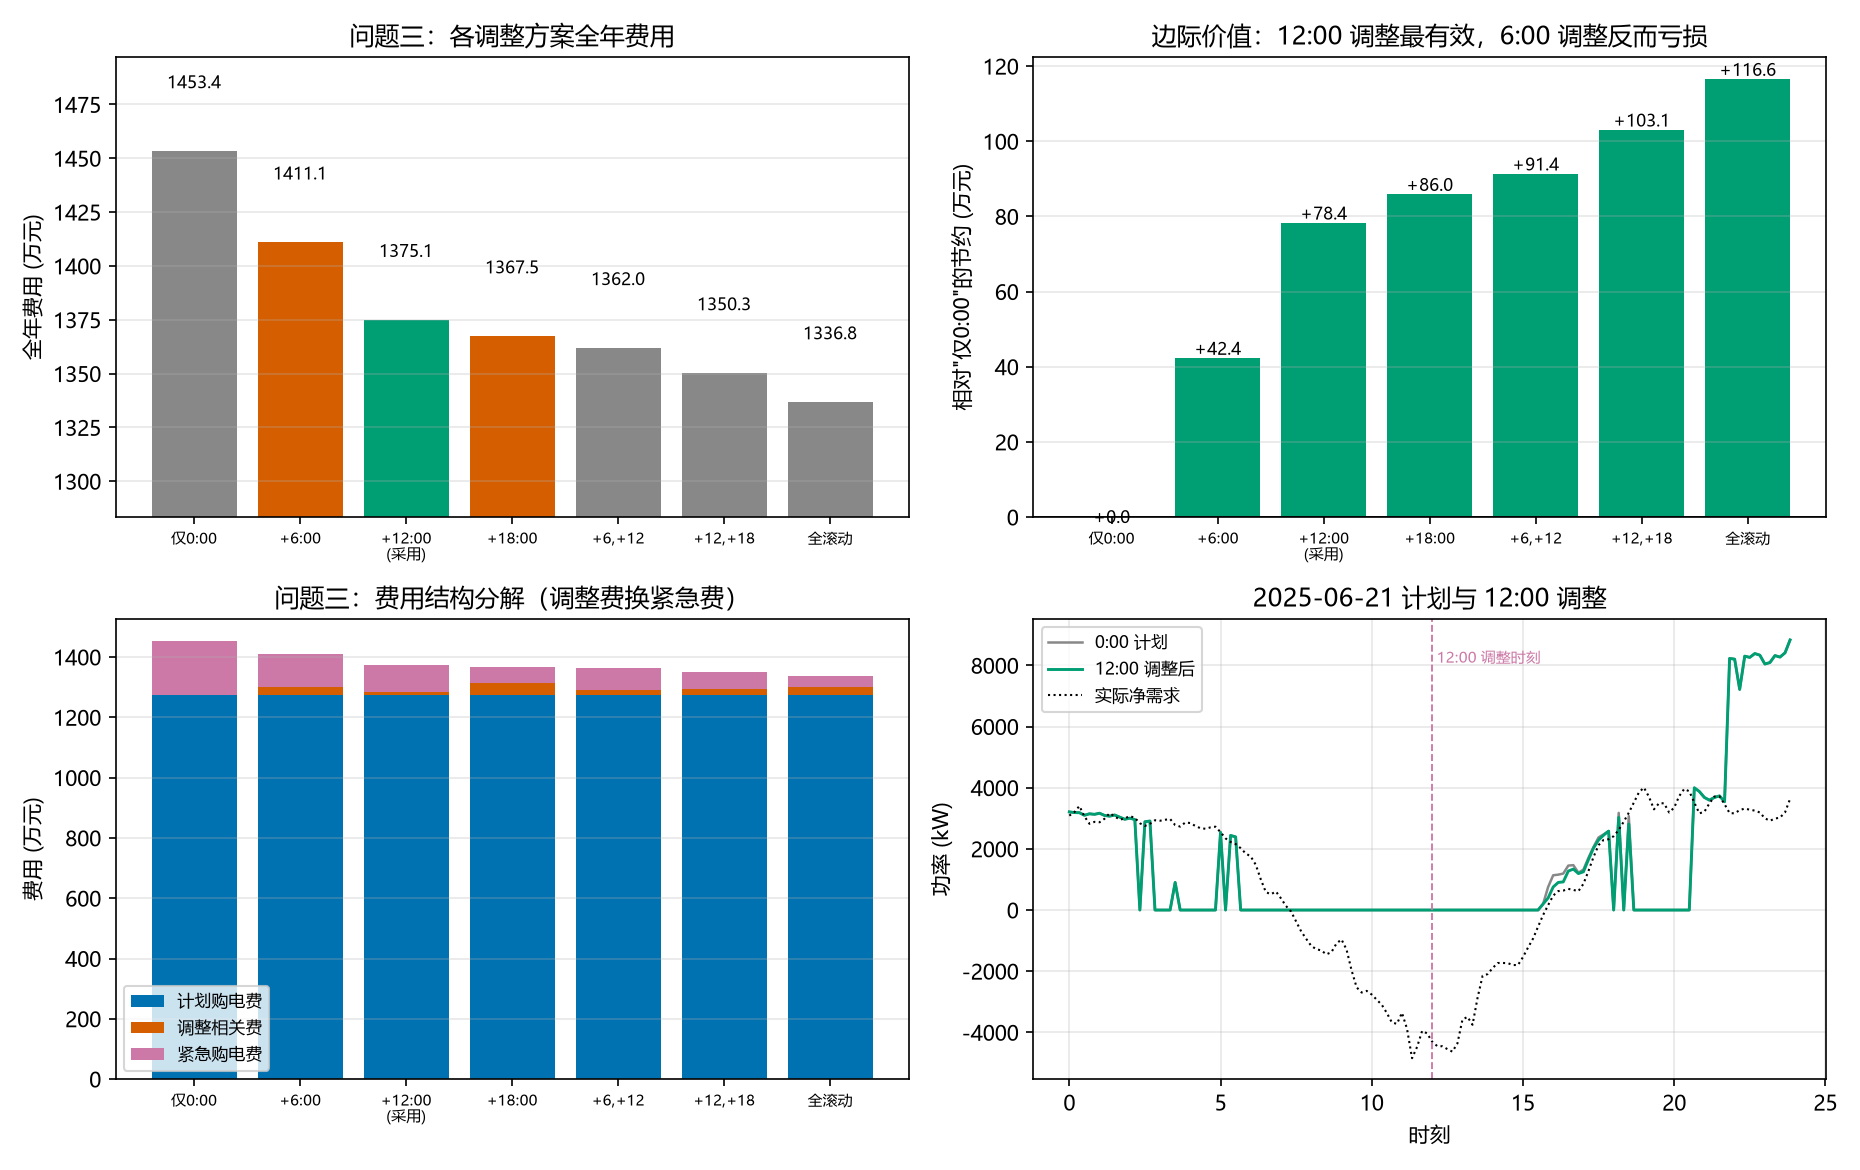
\includegraphics[width=0.95\textwidth]{figures/fig_q3_rolling.png}
\caption{问题三\nobreak：各调整方案全年费用（左上\nobreak）\nobreak、调整的边际价值（右上\nobreak）\nobreak、费用结构分解（左下\nobreak）\nobreak、
2025-06-21 计划与逐段调整（右下\nobreak）}
\label{fig:q3}
\end{figure}

\subsection{指定日期结果（表 1\nobreak、表 2\nobreak、表 3 格式\nobreak）}

\begin{table}[htbp]
\centering
\caption{问题三\nobreak：指定日期关键时段计划购电量与全天购电量\nobreak、购电费（表 1 格式\nobreak，kWh/元\nobreak）}
\label{tab:q3t1}
\zihao{-5}
\begin{tabular}{@{}lcccc@{}}
\toprule
时间段 & 2025-03-20 & 2025-06-21 & 2025-09-23 & 2025-12-21 \\
\midrule
10:00-10:10 & 0.00 & 0.00 & 0.00 & 0.00 \\
12:00-12:10 & 525.89 & 0.00 & 351.76 & 983.64 \\
14:00-14:10 & 0.00 & 0.00 & 0.00 & 0.00 \\
16:00-16:10 & 664.97 & 189.42 & 582.12 & 870.07 \\
18:00-18:10 & 698.46 & 0.00 & 788.53 & 713.64 \\
20:00-20:10 & 0.00 & 0.00 & 0.00 & 0.00 \\
\midrule
全天购电量 & 69\,256.54 & 36\,296.46 & 69\,316.87 & 96\,019.52 \\
全天购电费 & 42\,097.24 & 20\,517.82 & 43\,083.59 & 61\,259.08 \\
调整后全天购电量 & 66\,338.97 & 35\,914.80 & 66\,409.81 & 95\,903.74 \\
调整后购电相关费 & 42\,250.84 & 20\,338.79 & 42\,424.26 & 62\,089.51 \\
\bottomrule
\end{tabular}
\end{table}

\begin{table}[htbp]
\centering
\caption{问题三\nobreak：指定日期最终储能充放电量与 0:00\nobreak、24:00 储电量（表 2 格式\nobreak，kWh\nobreak）}
\label{tab:q3t2}
\zihao{-5}
\begin{tabular}{@{}lcccccccc@{}}
\toprule
\multirow{2}{*}{时间段} & \multicolumn{2}{c}{2025-03-20} & \multicolumn{2}{c}{2025-06-21} & \multicolumn{2}{c}{2025-09-23} & \multicolumn{2}{c}{2025-12-21} \\
\cmidrule(lr){2-3}\cmidrule(lr){4-5}\cmidrule(lr){6-7}\cmidrule(lr){8-9}
 & 充电 & 放电 & 充电 & 放电 & 充电 & 放电 & 充电 & 放电 \\
\midrule
0:00--4:00 & 133.26 & 208.53 & 104.74 & 3760.92 & 203.48 & 151.73 & 86.04 & 141.29 \\
4:00--8:00 & 83.20 & 6291.03 & 419.03 & 4838.06 & 224.13 & 6639.28 & 929.45 & 1509.97 \\
8:00--12:00 & 3949.46 & 2315.78 & 10\,092.26 & 0.00 & 5412.15 & 1896.62 & 5239.03 & 7811.29 \\
12:00--16:00 & 6398.23 & 372.51 & 0.00 & 0.00 & 5474.63 & 467.24 & 8133.72 & 2191.93 \\
16:00--20:00 & 212.45 & 5335.82 & 68.17 & 5701.03 & 92.29 & 5890.54 & 14.16 & 5917.13 \\
20:00--24:00 & 10\,715.90 & 2892.07 & 10\,045.62 & 2491.14 & 10\,562.50 & 2730.93 & 10\,666.67 & 2734.34 \\
\midrule
0:00 储电量 & \multicolumn{2}{c}{10\,800.00} & \multicolumn{2}{c}{10\,800.00} & \multicolumn{2}{c}{10\,669.60} & \multicolumn{2}{c}{10\,800.00} \\
24:00 储电量 & \multicolumn{2}{c}{10\,792.43} & \multicolumn{2}{c}{10\,800.00} & \multicolumn{2}{c}{10\,690.38} & \multicolumn{2}{c}{10\,800.00} \\
\bottomrule
\end{tabular}
\end{table}

\begin{table}[htbp]
\centering
\caption{问题三\nobreak：指定日期紧急购电时间段与购电量（表 3 格式\nobreak，kWh\nobreak）}
\label{tab:q3t3}
\zihao{-5}
\begin{tabular}{@{}llll@{}}
\toprule
2025-03-20（合计 559.67\nobreak） & 2025-06-21 & 2025-09-23（合计 419.00\nobreak） & 2025-12-21（合计 307.78\nobreak） \\
\midrule
9:00-10:00\ 461.60 & \multicolumn{1}{c}{无紧急购电} & 20:20-20:40\ 308.95 & 10:30-10:50\ 199.59 \\
20:30-20:40\ 84.84 &  & 20:50-21:10\ 98.80 & 20:30-20:40\ 108.19 \\
21:20-21:40\ 13.23 &  & 21:20-21:30\ 11.25 &  \\
\bottomrule
\end{tabular}
\end{table}

对比\cref{tab:q2t3} 与\cref{tab:q3t3} 可见\nobreak：逐段调整后 2025-09-23 的紧急购电量由
228.74 kWh 升到 330.42 kWh\nobreak、2025-12-21 由 31.13 kWh 降到 13.23 kWh\nobreak，
而 2025-03-20 由 54.68 kWh 升到 559.67 kWh（该日 12:00 的预报偏乐观\nobreak，计划量被下调\nobreak，风险后移\nobreak）\nobreak。
这与式 \eqref{eq:marginal} 的结论一致\nobreak：\textbf{调整的收益主要来自“按最新预报重新分配购电时段\nobreak”的
计划购电费变化与紧急购电费变化之差}\nobreak，个别日期紧急电量上升不代表调整变差\nobreak。
